\section{The Problem of Organizational Perspective Discovery}\label{sec:problemDescription}

The problem we address in this section is the discovery of the roles that members of a software project may actually play in a collaborative setting. Each member is assigned to at least one role in the project. Roles are decided in the project planning phase. This phase also involves the definition of project tasks and the assignment of suitable tasks to the various roles. 

Projects follow clear guidelines. Guidelines may come from internal policies or from rules and regulations of the working domain. For example, software systems in the railway domain must make sure that their development process and resources comply with safety requirements imposed by the European standard EN50128. This is why project managers need to track how they distribute work to different people and whether the project members effectively contribute according to their role and their task. 

\Gls*{scm} systems are a valuable source of information to investigate on the behavior of project members. These systems are used for tracking and controlling changes in the software. If a change produces a wrong or undesired outcome, it is always possible to revert to an older configuration of the system. Artifacts' versions are automatically managed by \glspl*{vcs}. It is always possible to follow the evolution of each artifact, along with information about the resources who changed it and their comments, by looking into the \gls*{vcs} logs.

\Cref{fig:big-picture} illustrates how people work in a project. People are assigned to defined roles and contribute to shared tasks or perform tasks alone. Their contributions are part of generated artifacts. As the project is enacted, the number and the content of the artifacts in a project grows. Changes in the artifacts themselves and in the structure of the project reflect the development process that project workers follow. The evolution of the repository mirrors the progress of the project.

\begin{figure}
   \centering

   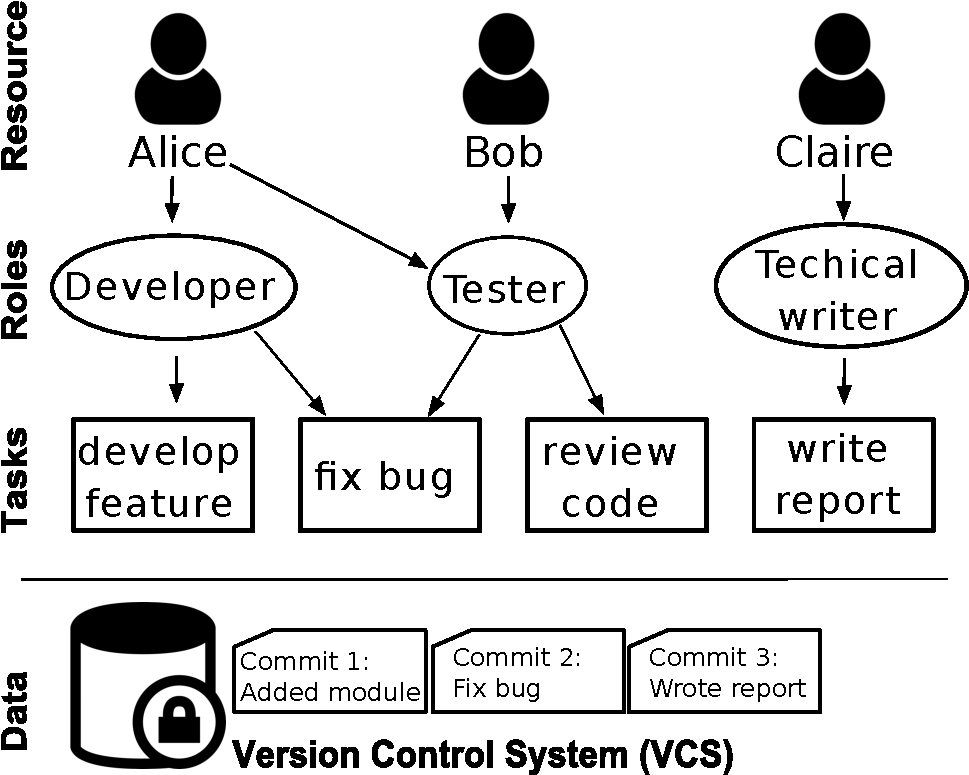
\includegraphics[width=.7\columnwidth]{ResourceClassification/figures/vcs3-crop.pdf}      
   \caption{Software project and resources}
   \label{fig:big-picture}
\end{figure}

\Gls*{vcs} logs provide rich and fine grained information about the changes in the project. 
A change may consist of a file being modified or new files being added to or removed from the repository. When changes are complete, it is possible to store them in the repository through a commit. Each commit contains a unique revision number, the identity of the resource who issued the commit, a timestamp, statistical information about the changes for each affected file, and a comment from the person who committed.

%A new commit moves forward the version of the files them were affected by the action of the user.
%Popular \glspl{vcs} are Git~\cite{torvalds2010git}, Mercurial~\cite{OSullivan2009} and SVN~\cite{pilato2008version}.

%Kushal's text
Let us consider the following example of how people use a \gls*{vcs} to collaborate in a project. Alice is a software engineer at Abc. ltd, and works on a project with her colleagues Bob and Claire. Alice is mainly assigned to the role \emph{developer}, but she can also be a \emph{tester}. Her tasks include the development of new features and fixing of related bugs. When a feature is ready she performs a commit and adds a new message where she describes her work, e.g. ``added new module to demo". At the same time she updates a file named ``rule''. This is reflected in the \gls{vcs} log, like in the first row of \Cref{tab:log-table-kushal}, identified by commit id 1. Bob is a \emph{tester} whose task is to ensure that the code submitted by Alice works properly. He discovers a bug in the ``setup'' interface file. Bob fixes those minor bugs and informs Alice of further work needed on the feature. Meanwhile, he commits his changes with commit id 2 and comments ``Modified the setup interface". Consequently, Alice reworks her code and commits a new version as reported in row 3 of \Cref{tab:log-table-kushal}, commenting her work with ``Update application interface". As a \emph{technical writer}, Claire takes over and starts to work on the documentation. She commits part of her work as in row 4. As the project continues, the work is accordingly stored in the log as in \Cref{tab:log-table-kushal}.

%\todo[inline]{\Cref{tab:log-table-kushal}: fill in with data from the running example}
%% Please add the following required packages to your document preamble:
% \usepackage{booktabs}
% \usepackage{multirow}
\begin{table}[]
\centering
\caption{Example of a \gls{vcs} log}
\vspace{5pt}
\label{tab:log-example}
\begin{tabular}{@{}cccll@{}}
   \toprule
   \textbf{ID}        & \textbf{Res}       & \textbf{Timestamp}                   & \textbf{Changelist} & \textbf{Comment}                                                                                 \\ \midrule
   \multirow{2}{*}{1} & \multirow{2}{*}{Y} & \multirow{2}{*}{2014-11-12 11:57:46} & A /file1            & \multirow{2}{*}{Added initial files}                                                             \\
   &                    &                                      & A /file2            &                                                                                                  \\ \midrule
   \multirow{2}{*}{2} & \multirow{2}{*}{X} & \multirow{2}{*}{2014-11-14 16:34:07} & M /file1            & \multirow{2}{*}{Developed interfaces}                                                            \\
   &                    &                                      & M /file2            &                                                                                                  \\ \midrule
   3                  & W                  & 2014-12-15 13:49:11                  & D /file1            & \begin{tabular}[c]{@{}l@{}}Reviewed interfaces. \\ Delete first. \\ Improve second.\end{tabular} \\ \midrule
   4                  & W                  & 2015-01-08 16:06:41                  & A /file3            & Added better interface                                                                           \\ \midrule
   \multirow{2}{*}{5} & \multirow{2}{*}{X} & \multirow{2}{*}{2015-01-13 11:47:09} & M /file2            & Improve backend                                                                                  \\
   &                    &                                      & M /file3            & Add feature                                                                                      \\ \midrule
   \multirow{2}{*}{6} & \multirow{2}{*}{Z} & \multirow{2}{*}{2015-01-16 16:50:29} & A /file4            & \multirow{2}{*}{Added tests}                                                                     \\
   &                    &                                      & A /file5            &                                                                                                  \\ \bottomrule
\end{tabular}
\end{table}
\begin{table*}[]
\centering
\caption{Example of a \glstext{vcs} log in the context of Organizational Perspective Discovery}
\label{tab:log-table-kushal}
   \begin{tabular}{m{0.5cm}m{1cm}m{3cm}m{2cm}m{4.5cm}}
%      \toprule
      \rot{\textbf{Commit ID}} & \rot{\textbf{User ID}} & \textbf{TimeStamp}  & \textbf{Updated Files}                                        & \textbf{Comment}                                         \\ \midrule
      1                  & Alice            & 2014-10-12 13:29:09 & \begin{tabular}[c]{@{}l@{}}Demo.java\\ rule.txt\end{tabular}   & Added new module to demo and updated rules               \\
      2                  & Bob              & 2014-11-01 18:16:52 & Setup.exe                                                     & Modified the setup interface                             \\
      3                  & Alice            & 2015-06-14 09:13:14 & Demo.java                                                      & Update the application interface                         \\
      4                  & Claire           & 2015-07-12 15:05:43 & \begin{tabular}[c]{@{}l@{}}graph.svg \\ todo.doc\end{tabular} & Define initial process diagram \& listed remaining tasks \\
      \ldots                  & \ldots              & \ldots & \ldots                                                     & \ldots                                                  \\ 
%      \bottomrule
   \end{tabular}
\end{table*}

As we can see from the example, user work is tracked in a fine granular way by the \gls{vcs}. The challenge is to use log information for getting insights into the roles of project members. The following section discusses related literature that has addressed role discovery.

%\subsection{Version Control Systems}
%
%A VCS is an application with the purpose of tracking changes in documents. The most common example of such a document is source code of software, but it can also be natural language text, structured text content or any other kind of information. Each change of a file creates a new version or revision of this file.
%
%
%All versions are stored in a repository and can be accessed for different purposes, for example to switch to an older version, to find out which user made a certain change or to revert the document to a previous state. A commit is a collection of file changes passed to the VCS at once by a single user. Usually users provide a message for each commit, which describes the contributed changes. A VCS log is a chronological history of commits. The information included in these logs depends on the VCS and can be configured. It usually includes for each commit some kind of identifier, the author, a timestamp, the commit message and the number of added, modified and deleted files. The most commonly used systems for software development are Git~\cite{torvalds2010git}, Mercurial~\cite{OSullivan2009} and SVN~\cite{pilato2008version}.
%
%
%Version control systems can be used within companies to enable the individual employees to work together on projects. Tasks are distributed and the results then have to be merged to create the product. This can be done via commits in a VCS. It documents the current status of the project and changes have to be committed into the repository. Conflicts, due to multiple users working on the same resource, have to be resolved and the VCS creates a history, where every change can be tracked. Additionally, the users can try out their ideas on their own systems without breaking the whole project.
%
%
%The VCS also keeps a history of all versions. Customers receive a certain product version and for bug fixes for this specific version only the version id is required, instead of maintaining a copy for each customer. For open source projects it enables users to work around the world at any time, while enabling new workflows. Additionally, the entry barrier for new users is lowered. Downloading the repository, applying changes and committing them, even if he /she only once advances the project, can be done by anyone. 
%
%
%\subsection{User Classes}
%
%There are various types of user classes. The most apparent interpretation are classes corresponding to typical official or implicit roles within a software project (e.g. developer, tester...). But there are also other possible ways of classification, such as by individual experience, age of users, distinction in supervisor, subordinate relationships commitment, commitment and various demographics or personality traits. This research focuses on the project roles but additional classifications are not excluded.
%
%There is a large number of roles in software development
%
%proposed and analyzed by literature. Roles relevant for this context have to be identified, meaning that these roles create commits at all and that they provide some kind of characteristics to identify them. The identified roles which fulfill these conditions are: developer (can be split up into backend, frontend or web developers), tester, designer, technical writer, architect, toolsmith, database expert and (VCS or build) administrator (Acua \& Juristo, 2004) (Shore, 2007).
%
%However, especially in smaller teams and projects it is quite common that a single user has multiple roles.  In some cases these roles are formally defined, in others they are just reflected by the tasks and responsibilities of the user. Especially in open source projects there is often no explicit separation of roles.

%\subsection{Requirements}

As mentioned in the previous section, the focus of this section lies on mining and analyzing properties of the users of \gls{vcs}. Users belong to preset classes and they commit message styles. Based on this assumption, the following requirements are defined.

\begin{itemize} %\IEEEsetlabelwidth{Z}
      
\item[\textbf{RQ1. Cluster users from event log.}] 
We want to provide a classification of the users of a \gls{vcs} by using the information contained in the log files. Comment messages and other data must be investigated for useful features. The classification must separate the users into clusters, and the most expressive features and their combinations must be identified.  These clusters can then be further analyzed by means of the next research question.

\item[\textbf{RQ2. Create user profiles.}]
Based on the created clusters, meaningful classes should be derived. The chosen features influence the types of classes that can be created. These classes must present an intelligible distinction among each other. This requirement aims at making class distinctions clear-cut. Moreover, it aims at creating profiles for the class members reflecting behavior, based on the analyzed features.

\item[\textbf{RQ3. Generalize approach.}]
The last research question examines the differences among the created classes in detail. It compares the results from different log files and identifies the reasons for dissimilarities. Therefore, it evaluates the quality of the classification and its applicability for different version control systems.

\end{itemize}


\subsection{Related Work}
Role discovery has been addressed by literature in different settings and from several points of view. Here we highlight existing efforts from a data perspective.

\subsubsection{Structured data approaches}
This class of methods includes algorithms that make use of quantifiable data. We divide them into: 
\begin{inparaenum}[\itshape a)]
   \item \gls*{msr} approaches; and
   \item \gls*{pm} approaches.
\end{inparaenum}

\paragraph{\bfseries Mining software repositories approaches}
In the area of \gls*{msr}, \cite{Yu.LiguoRamaswamy.2007} use a hierarchical clustering based on user interactions to identify two categories of users: \emph{core member} and \emph{associate member}. Core members are those users whose interaction frequency is higher than a given threshold. Associate members are instead users whose interaction frequency is below the threshold.
\cite{Alonso2008} use a rule-based classifier that maps file types onto categories and hence each author who modified a file is linked to the files' category. ~\cite{gousios2008measuring} classify developers contribution based on \gls*{loc} changes and infer activities from them. \cite{Begel2010} developed the Codebook software tool a utility for finding experts. They use a social network approach that combines sources from people, artifacts, and textual references to other people. 
%Codebook is able to crawl several repositories and store the data as a graph in a database. Using a social network approach, that combines sources from people, artifacts, and as well as textual allusions to other people, this tool allows for finding experts. 
\cite{Ying2014} study developer profiles in terms of their interaction with the software artifacts to understand how they modify files and to further recommend changes based on history from \gls*{vcs} logs. \cite{Fuller2014a} investigate user roles in innovation-contest communities. They use quantitative methods to analyze user activity logs and interpretative to categorize qualitative comments into classes. 
%Furthermore, they used clustering to identify six user types: master, idea generator, socializer, efficient contributor, passive idea generator, passive commentator. Their work point out that different users are indeed characterized by behavioral contribution patterns. 

\paragraph{\bfseries Process mining approaches}
Efforts have been done to analyze software repositories with process mining techniques. \cite{rubin2007process} implement a multi-perspective incremental mining that is able to continuously integrate sources of evidence and improve the software engineering process as the user interacts with the documents in the repository. Their approach allows for mining other perspectives, such as roles, by applying social network analysis. However, only statistical methods can be applied to their output, since it lacks the comments that are associated to file changes. In the same setting, \cite{DBLP:conf/csmr/PoncinSB11} developed \textsc{frasr}, a framework for analyzing software repositories. \textsc{frasr} can be used in order to transform \gls*{vcs} logs data into the XES~\citep{verbeek2010xes} data format that can be further analyzed with process mining tools like ProM\footnote{http://www.promtools.org/doku.php}. 
\cite{Song2008} focus on three types of organizational mining 
\begin{inparaenum}[\itshape i)]
   \item organizational model mining, 
   \item social network analysis, and 
   \item information flows between organizational entities.
\end{inparaenum} 
\cite{Schonig2015} propose a mining technique to discover resource-aware declarative processes.

\subsubsection{Unstructured data} \cite{Maalej2010} use \gls*{nlp} for automating descriptions of work sessions by analyzing developers' informal text notes about their tasks. Developers are then classified into two classes based on their behavior: developers who use problem information to refer to their current activity and developers who refer to task and requirements. \cite{Kouters2012} developed an identity merging algorithm based on Latent Semantic Analysis (LSA) to disambiguate user emails. \cite{Licorish2014} mined developer comments to understand their attitudes.

\subsubsection{Other related work} The term \emph{role mining} often points to role mining algorithms based on \gls*{rbac} systems. These algorithms take as input predefined roles that are given as a matrix, where each user is assigned to access permissions. A number of algorithms have been developed to mine roles from \gls*{rbac} systems alone \citep{Lu2015,frank2013role} or combining their data with process history logs, as in \citep{baumgrass2012deriving}. A survey of existing techniques and algorithms can be found in \citep{Mitra2016}. Our work is disjoint from this class of algorithms as \gls*{vcs} does not contain access control information. 
\cite{Bhattacharya2014} propose a contributor graph-based model. By constructing a source-based profile, and a bug-based profile, they are able to identify seven roles: \emph{patch tester}, \emph{assist}, \emph{triager}, \emph{bug analyst}, \emph{core developer}, \emph{bug fixer}, and \emph{patch-quality improver}. \cite{hoda2013self} use a \gls*{gt} approach to study agile teams. Their work distinguishes the roles of \emph{mentor}, \emph{coordinator}, \emph{translator}, \emph{champion}, \emph{promoter}, and \emph{terminator}.


This work builds upon existing literature in that it strives to get insights on organizational level like in \cite{rubin2007process} and \cite{Song2008}, but it takes into account unstructured data. Differently from the literature that works with unstructured data, we explicitly consider the problem of role discovery, i.e. label resources with roles. Lastly, this approach differs from \cite{Bhattacharya2014} and \cite{hoda2013self} since we further adopt \gls*{nlp} techniques.

